\chapter{Word stress in Tashlhiyt}
\section{Word stress: a working definition}

While there are many claims that ‘word stress’ (or ‘lexical stress’) is a universal feature of human languages (e.g. \citealt{GoedemansVanderHulst2009}), the universality of this linguistic phenomenon very much depends on how it is defined. Following the main assumptions of the Autosegmental-Metrical (AM) model, word stress shall be defined as an abstract strength relationship between syllables at the level of the phonological word, as reflected in Hyman’s definition (\citealt{Hyman2014}):

\begin{exe}
\ex\label{ex:4:1} Word stress refers to the phonological marking of one most prominent syllable of the phonological word.
\end{exe}

This definition crucially presupposes the presence of two linguistic units: the syllable and the phonological word, two units that, although very common cross-linguistically, have been claimed not to be universal. \citet{Hyman2011} analysed Gokana, a Gogoni language spoken in Nigeria, as exhibiting no linguistic evidence for the syllable as a relevant linguistic unit. \citet{Schiering.etal2010} discuss evidence from Vietnamese and Limbu that suggests that the phonological word is not a universal prosodic domain either. However, since both the syllable and the word have been argued to be relevant linguistic units in Tashlhiyt (e.g. \citealt{DE2002,Ridouane2008}), we proceed by assuming that the proposed definition of word stress is applicable.\il{Gokana}\il{Vietnamese}\il{Limbu}

Proposing abstract strength relationships within the word needs to be empirically justified. Prototypically, word stress systems are described as exhibiting some of the following phonological properties: the word stress position is phonemic; stressed syllables exhibit greater segmental or tonal contrasts and usually undergo lengthening processes, while unstressed syllables exhibit fewer contrasts and usually undergo shortening processes; stressed syllables are phonetically enhanced; stressed syllables co-occur with postlexical tonal events.

In English\il{English}, stress has been analysed as phonemic (e.g. \citealt{HalleVergnaud1987,Hayes1995}). In \REF{ex:4:2}, the noun \textit{import} is distinguished from the corresponding verb by the position of the stressed syllable only. In English, stress is also frequently associated with a process of vowel reduction. Unstressed syllables are often produced with reduced vowels or syllabic consonants in syllable nucleus position. Example \REF{ex:4:3} demonstrates the alternation of stressed /ɒ/ in \textit{harmonic} and unstressed /ə/ in \textit{harmony}. The reduction of unstressed vowels results in a smaller vowel inventory in unstressed syllables than in stressed syllables.

\begin{exe}
\ex\label{ex:4:2} import, \textsc{n} /ˈɪm.pɔːt/ vs. import, \textsc{v} /ɪm.ˈpɔːt/
\ex\label{ex:4:3} harmonic /hɑː.ˈmɒ.nɪk/ vs. harmony /ˈhɑː.məṇi/
\end{exe}

In addition to qualitative differences, stressed syllables are often phonetically enhanced. The phonetic correlates of stress are typically investigated via measurements of duration, intensity, and fundamental frequency (cf. \citealt{Fry1955,Fry1958}, for a recent overview see \citealt{Gordon2014,GordonRoettger.underreview}). Most languages exhibit increased duration, greater intensity, higher fundamental frequency, or some combination of these as acoustic markers of stress. However, although stress is often correlated with phonetic enhancement, some languages exhibit ambiguous phonetic cues as to which syllable is the most prominent. For example, stressed syllables in Modern Welsh have been reported to exhibit shorter vowel durations than vowels in unstressed syllables (\citealt{Williams1999}).\is{word stress}

Moreover, cross-linguistic phonetic studies that have investigated word stress in the past have frequently used methodologies that do not allow word-level phonetic prominence to be distinguished from prominence attributable to higher prosodic constituents. For example, many studies rely on acoustic records of words that are read out from lists making it impossible to disentangle word stress from phrasal phenomena. It is thus crucial for an evaluation of word-level stress in any language to tease apart different levels of prosodic structure (for an overview see \citealt{RoettgerGordon.underreview}).\is{word stress}

Related to the last point, stressed syllables can interact with postlexical events and can be the designated elements for the association of intonational tones, i.e. pitch accents (or phrase accents, cf. Chapter 2). In English\il{English}, pitch accents are associated with stressed syllables, i.e. they systematically co-occur with the metrically strong element of prominent words in the phrase. Recall the incredulity example in Chapter 2 (\figref{fig:2.3}, \textit{A statistics instructor!?}). Alongside an utterance-final rise, this contour is characterised by a rise and subsequent fall around the metrically strongest syllable in the compound. Although stress is often correlated with the co-occurrence with intonational tones, it does not constitute a sufficient argument in itself for the presence of word stress. Whilst in English, pitch accents go hand in hand with stressed syllables, this is not necessarily the case for other languages (for an overview see \citealt{Gordon2014}). For example, as discussed in Chapter 2, phrase accents are sometimes associated with specific syllables close to a phrase boundary that are not necessarily lexically stressed (\citealt{Grice.etal2000}).\is{word stress}\is{pitch accent}

In the following, we will discuss possible evidence for the notion of word stress in Tashlhiyt. We will argue that there is no convincing phonological evidence for lexically determined stress in this language. Although a recent study presented phonetic evidence for systematic phonetic prominence asymmetries within the word (\citealt{GordonNafi2012}), we will argue that these findings are likely the result of post-lexical phenomena (\sectref{sec:4.2}). Subsequently, we will present a production study that provides evidence for the null, i.e.\ there are no lexically specified prominence asymmetries within the word (\sectref{sec:4.3}) leading to the conclusion that there is no word stress in Tashlhiyt. Finally, these results will be discussed in context of comparable languages that have been claimed to lack word stress (\sectref{sec:4.4}).

\section{Evidence for word stress in Tashlhiyt}\label{sec:4.2}
\subsection{Early observations}
Early descriptions of Tashlhiyt have claimed that ‘stress’ is only found in utterance final position:

\begin{quote}
[…] stress patterns referred to here apply only to utterances consisting of a single word. If the utterance contains more than one word, the stress is reduced slightly on all vowels except those in the final word. It can be said, therefore, that primary stress occurs only at the end of an utterance. (\citealt[9]{Applegate1958})
\end{quote}

It has further been claimed that stress in Tashlhiyt is likely to be a phenomenon of higher prosodic constituents rather than the word:

\begin{quote}
Whereas in an English\il{English}\il{Italian} or Italian sentence every polysyllabic word has its own prominence peak, it is highly dubious that the same obtains in Imdlawn Tashlhiyt. If Imdlawn Tashlhiyt has a phenomenon that could be called stress or accent, it is likely that it is a property of units larger than words. (\citealt[14]{DE2002})
\end{quote}

These authors acknowledge the presence of certain prominence asymmetries at the phrase level. The authors also make it very clear that there is a distinction to be made between the notion of word stress and the prominence phenomena attributed to higher levels of prosodic organisation.\is{word stress}

In Tashlhiyt, there is no evidence for a phonologically marked prominent syllable in the domain of the phonological word: there are no known phonotactic restrictions on certain syllable positions, i.e. all syllable positions within a word allow the same inventory of phonemic contrasts. To my knowledge, there is no grammatical pattern that takes phonologically prominent syllables into account (in line with observations made by Kossman, p.c. February 2015). Generally, there are few, if any, minimal pairs solely distinguished by phonetic prominence, and speakers report that they confuse these (Ridouane, p.c. October 2013). \citet{Stumme1899} notes that word ‘accent’ usually falls on the word stem but that it can be shifted by certain word formation processes. Similarly, \citet{Sadiqi1997} notes that stress is not distinctive, however, she proposes that word stress falls on the last vowel of the stem if there is no suffix following. These  observations, however, are not supported by experimental evidence.

Moreover, speakers are rather insensitive to phonetic prominence asymmetries within the word. In line with my own experiences, \citet[708]{GordonNafi2012} state explicitly that speakers are not able to consistently identify a syllable as being stressed, neither through direct questioning nor through rhythmic tasks in which speakers had to tap their finger when producing a stressed syllable.\is{word stress}

\subsection{Gordon and Nafi (2012)}
Despite the lack of clear phonological evidence and the absence of any indication of native speakers’ awareness of stress, \citet{GordonNafi2012} have recently argued that Tashlhiyt does indeed have word-level prominence, namely on the final syllable of the word. They investigated three acoustic correlates of prominence: duration, intensity, and mean fundamental frequency. They recorded six participants that read out di- and trisyllabic target words in two different contexts: (i)~in isolation, resulting in the target word forming its own intonation phrase, and (ii) followed by an adverb, resulting in the target word being in phrase-medial position. Target words were selected to cover a wide range of phonotactic patterns with syllables having vowels (e.g. /ba.lak/ ‘Get out of the way’), sonorant consonants (e.g. /t.zm̩.zm̩/ ‘She squeezed’) or obstruents (e.g. /tf̩.tk̩t/ ‘She sprained it’) in syllable nucleus position.

The authors found that phrase-final nuclei consistently had higher f0 values than other syllables. However, they interpreted this as a reflex of an intonational tone associated with a lexically strong final syllable in the target word. Irrespective of f0, they found that the syllable nuclei of word-final syllables, especially in phrase-final position, exhibited greater duration and intensity than the nuclei in penultimate syllables. This asymmetry between penult and final syllable has been reported to be robust for vowels (analysis based on two word pairs, n=2) and sonorants (based on n=5). The results were less convincing for obstruents (based on n=6), with no duration differences for voiced obstruents (n=2), and no intensity differences for voiceless obstruents (n=4). Since Gordon and Nafi’s study is the only study available that has looked at potential word-level prominence instrumentally, it is necessary to critically evaluate their findings. There are two major methodological concerns:\is{word stress}\is{pitch accent}

First, any prominence asymmetries found in their study might ultimately be triggered postlexically, a caveat they acknowledge in their paper. Durational asymmetries in final syllables might be due to postlexical strengthening phenomena such as final lengthening (e.g. \citealt{BeckmanEdwards1990,Edwards.etal1991,GussenhovenRietveld1992,Cho2005}), where lengthening at higher domains (intonation phrase final) is greater than at lower domains (e.g. word final). Although there is no direct instrumental evidence for final lengthening in Tashlhiyt, such asymmetries may explain the results on phrase-final syllables by \citet{GordonNafi2012}.

Orthogonal to the possibility of phrase-final lengthening, both longer durations and higher intensity in the final syllable may be postlexically triggered by tonal events. As Gordon and Nafi acknowledge, the final syllable appears to bear a tonal event, which the authors analyse as a “pitch accent”. (We will come back to the classification of these tonal events in Chapter 7). The point to be made here is that a postlexically relevant tonal event is located at the right edge of the utterance. This tonal event may be accompanied by phonetic enhancement, in line with numerous studies on pitch accents and phrase accents in other languages (e.g. \citealt{Harrington.etal2000,Cole.etal2007,Katsika.etal2014}). This phonetic enhancement of syllables co-occurring with tonal events in Tashlhiyt has been impressionistically described in \citet{Grice.etal2015tash}. This applies to syllables at the right edge of the utterance, but also to the final syllable of phrase-medial words (\citealt{RoettgerGrice2015}). In Gordon and Nafi’s study, speakers produced different target words in a constant carrier phrase, thus the target words were implicitly contrasted. Previous findings on Tashlhiyt by \citet{Grice.etal2011} have demonstrated that implicitly contrasted target words in phrase-medial position are realised with a pitch peak on the target word. This tonal event appears to prefer the right edge of the word, which could have been the source of the observed asymmetries in \citet{GordonNafi2012}.\is{word stress}\is{pitch accent}\is{focus}

 
Second, there are statistical concerns with Gordon and Nafi’s study. The authors analyse their data with analyses of variance (ANOVA) using speakers as the population that is inferred over, i.e. they average over different words. However, any claim that a language behaves in a certain way should be a robust generalisation not only over speakers but also over the lexicon, i.e. over the words of the language. Ignoring one of these levels and generalising, for example, only over speakers of a language, might result in a false positive. This statistical shortcoming has been described as the “language-as-fixed-effect fallacy” (\citealt{Clark1973}; see \citealt{Winter2011}, for a discussion related to phonetic research and \citealt{RoettgerGordon.underreview} for a discussion related to acoustic studies on word stress). Crucially, when claiming that a language has a fixed word stress position, any statistical generalisation must apply to the population of words. As was criticised by Clark more than forty years ago, statistical inference is often only made over speakers/listeners. Gordon and Nafi used a very limited set of target words. This makes generalising over the Tashlhiyt lexicon conceptually (and mathematically) not feasible.\is{word stress}

\section{Production study: Word stress in Tashlhiyt revisited}\label{sec:4.3}
This section presents data designed to address the above-mentioned methodological concerns and offers an answer to the question as to whether Tashlhiyt exhibits phonetic prominence asymmetries at the word level or not. To this end, a corpus was designed in which potential word-level prominence is not confounded with any postlexical events. Moreover, statistical methods were used that allow generalisation over both speakers and words of the language.\footnote{Parts of the presented experiment have been published in \citet{Roettger.etal2015}.}\is{word stress}

If we ignore the absence of phonological arguments in favour of word stress and assume that Tashlhiyt indeed has fixed word stress on the final syllable, it is hypothesised that there is a consistent acoustic prominence asymmetry between penultimate and final syllables. Alternatively, word stress may not be fixed in Tashlhiyt, i.e. different words may have different word stress positions.

\subsection{Method}
To test these hypotheses, short mock dialogues produced by ten speakers were analysed. Disyllabic target words appeared in three different sentences in phrase-medial position (cf. \ref{ex:4:4}--\ref{ex:4:6}, target words highlighted in bold). 

\begin{exe}
\ex\label{ex:4:4} is inna \textbf{baba} ʁakudan? \\
‘Did he say ‘father’ then?’
\ex\label{ex:4:5} uhu, inna \textbf{dari} ʁakudan. \\
'No, he said ‘in my house’ then.’
\ex\label{ex:4:6} inna target \textbf{dari} ʁakudan? \\
‘He said ‘in my house’ then?’
\end{exe} 

These sentences were designed to elicit specific intonation patterns: the first context was a yes-no question \ref{ex:4:4}, followed by a negation (/uhu/), and a contrastive statement \ref{ex:4:5} with the target word in corrective focus. The statement in \ref{ex:4:5} was followed by a confirmation-seeking echo question \ref{ex:4:6}. As will be further elaborated on in subsequent chapters, the target word in \ref{ex:4:5} is contrastively focused and is expected to co-occur with a rise in pitch followed by a fall. Echo questions are also expected to co-occur with a rise-fall in pitch but at the right edge of the utterance-final word. Crucially, in \ref{ex:4:6}, the target word is given information and not marked by any apparent tonal movement (cf. \figref{fig:4.1}).\footnote{The corresponding sound file of this contour and all following contours that are illustrated in figures throughout the rest of this book can be found at https://doi.org/10.5281/zenodo.815840.} This enables us to disentangle word-level prominence from postlexically induced prominence. \is{word stress}\is{yes-no question}\is{echo question}\is{focus}

\begin{figure}
  \centering 
   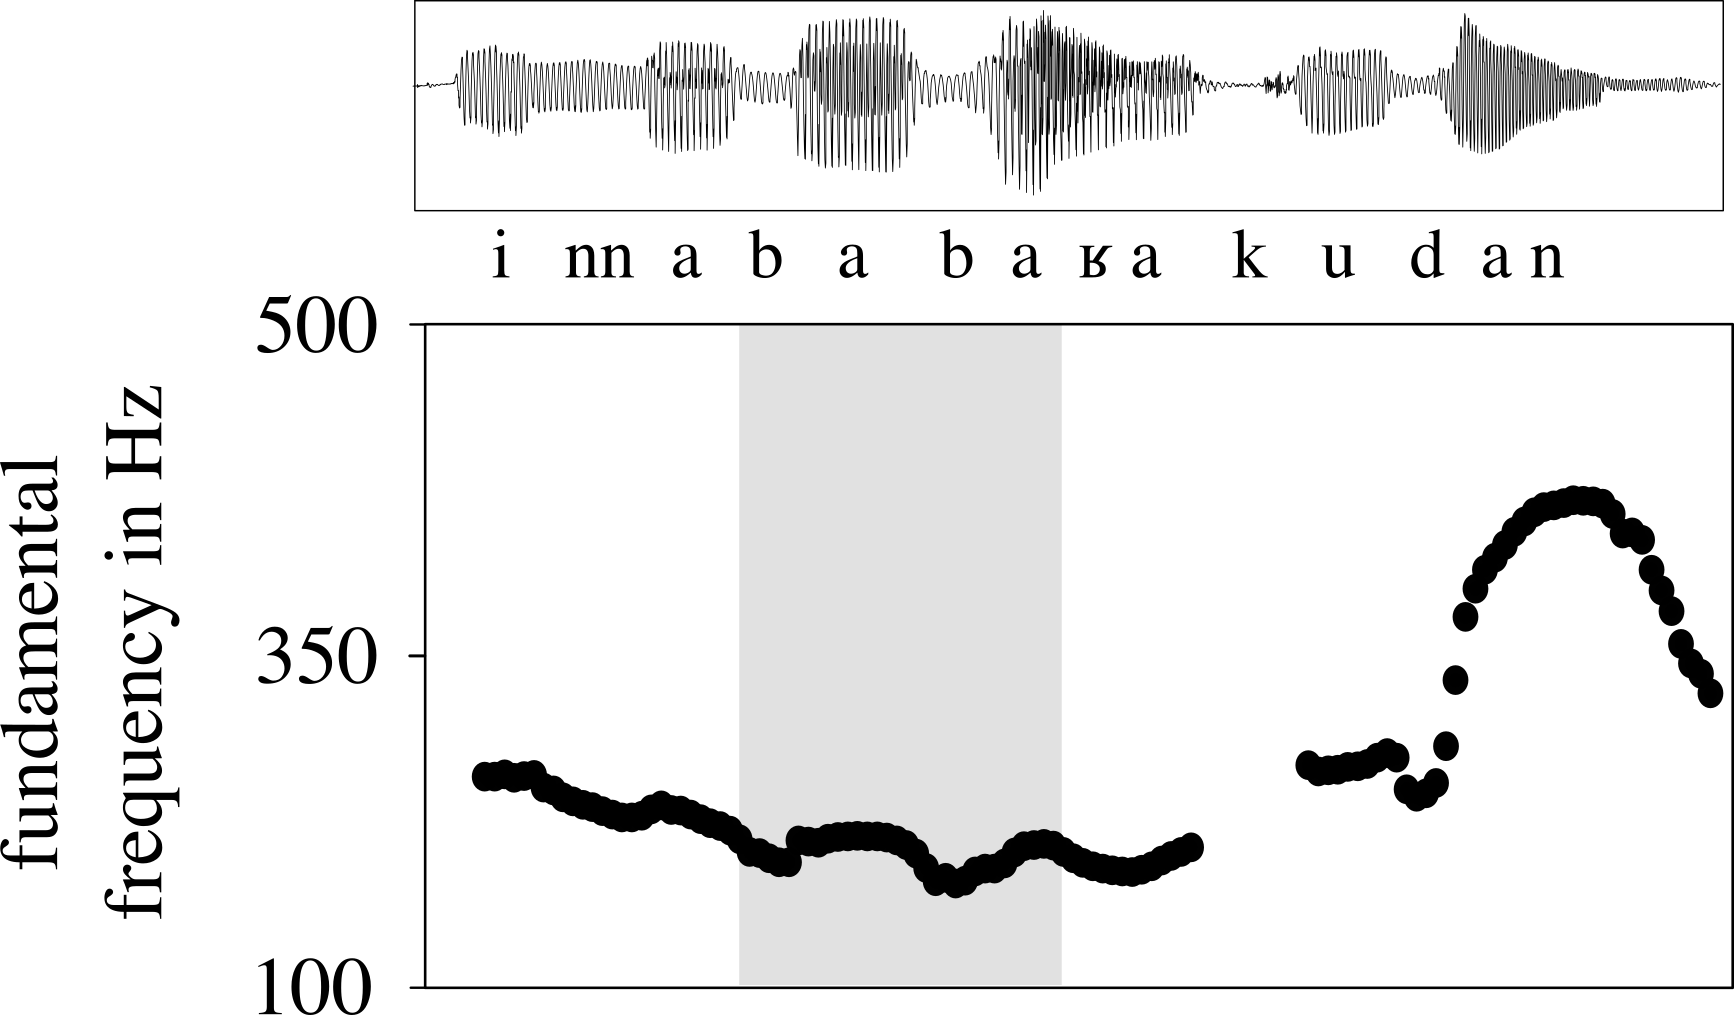
\includegraphics[width=0.7\textwidth]{figures/Figure_4_1.png}
  \caption{Representative waveform and f0 contour for the echo question /inna baba ʁakudan/ ‘He said ‘father’ then?’ The target word is highlighted in grey. Note that there is no apparent tonal event on the target word.}
   \label{fig:4.1}
   \end{figure}

\subsubsection{Participants and procedure}
Ten native speakers of Tashlhiyt (6 male, 4 female, mean age = 25, age range: 21-34) were recorded in Agadir in November 2014. One male speaker had to be excluded from the acoustic analysis due to malfunction of the recording device. All speakers live in Agadir, are fluent in Moroccan Arabic, and have a basic command of French (cf. Appendix A2.1 for participant information). Participants were asked to reenact orthographically presented mock dialogues (in Latin script) presented in cartoon form. Speakers were instructed to produce the dialogues as presented in \ref{ex:4:4} to \ref{ex:4:6}. Each target word was produced twice in each sentence modality by each speaker.

\subsubsection{Speech material}
A corpus of disyllabic target words was created. All target words were comprised of syllables with a vocalic element in syllable nucleus position. There were some words (n=6) containing two identical syllables (e.g. /baba/ ‘father’), such that the target syllable occurs in both penultimate and final position. The other word pairs (n=5) contained non-identical syllables, with the target syllable occurring once in penultimate and once in final position (e.g. compare the target syllable /di/ in /sidi/ ‘sir’ and /dima/ ‘always’). This resulted in 11 comparable target syllables. There were words containing light and heavy syllables, but only syllables with the same syllable weight were compared, i.e. light with light and heavy with heavy (as opposed to \citealt{GordonNafi2012}). These target words were presented alongside 14 obstruent-only filler words that are not further analysed here. All target words are displayed in \tabref{tab:4.1}.\is{syllable weight}

\begin{table}
  \begin{tabular}{ccc}
    \lsptoprule
    \textbf{Target word (1)}  & \textbf{Target word (2)}  & \textbf{Target syllable} \\
    \midrule
tama ῾next to᾽ & ʃita ῾brush᾽ & ta \\
dari ῾in my house᾽ & juda ῾enough᾽ & da \\
dima ῾always᾽ & sidi ῾sir᾽ & di\\
tili ῾ewe᾽ & hati ῾here is᾽ & ti\\
nizi ῾of the fly᾽ & ʁuni ῾sing᾽ & ni\\
baba ῾father᾽ &	& ba\\
bibi ῾turkey᾽ & & bi\\
kawkaw ῾peanuts᾽ & & kaw\\
kifkif ῾it is the same᾽ & & kif\\
tamtam ῾drum᾽ &	& tam\\
janjan ῾one-one᾽ & & jan\\
\lspbottomrule
  \end{tabular}
  \caption{Target words (in IPA) and translations. Note: the target word /ʁuni/ is borrowed from Moroccan Arabic (Tashlhiyt: /ʁnni/). The inclusion of this target word in the design was due to a misunderstanding with our consultant. The presented statistical analyses hold even after exclusion of this item.}
  \label{tab:4.1}
\end{table} 

\subsubsection{Analysis}
Only target words in echo questions were considered in the following analysis. All these target words were predicted to be realised with no pitch peak on the target word, allowing us to analyse prominence asymmetries at the word level, with no influence of the phrase level. This prediction was confirmed by the author via auditory and visual inspection of the f0 contour. Target words in echo questions were segmented and annotated with Praat 5.4 (\citealt{Praat2015}). All acoustic material was manually annotated employing the following labelling criteria: segment boundaries in the target words were identified in the acoustic waveform by means of an oscillogram and a wide-band spectrogram. All segmental boundaries of vowels and consonants were labelled at abrupt changes in the spectra indicating closure formation or release: this was the case for nasals, laterals (especially in the spectra for the intensity of higher formants), and obstruents (at random noise patterns in the higher frequency regions). To compare the data to Gordon and Nafi’s study as closely as possible, duration, average intensity, and average fundamental frequency for each target syllable nucleus were extracted. All data were analysed using R (\citealt{R}) and the “lme4” package (\citealt{Bates.etal2014}). The continuous variables nucleus duration (ms), mean nucleus intensity (dB), and mean fundamental frequency of the nucleus (Hz) were analysed with linear mixed effects models.\is{echo question}

Again, to evaluate our data against Gordon and Nafi’s analyses, a subject-based (averaging over all syllables) and a syllable-based analysis (averaging over all speakers) were performed. The predictor was syllable position (penult, henceforth “PU” vs. final syllable, henceforth “F”). Contrasts were deviation coded. In line with Gordon and Nafi’s analyses varying intercept-only models were used, i.e. we account for different speakers and different syllables having general higher or lower values for the respective parameter. In other words, this analysis tries to replicate Gordon and Nafi’s analysis in the most anti-conservative way. If no effect is found, we can be certain that the analysed acoustic parameters do not vary as a function of syllable position. However, if an effect is found, the results will be subject to further scrutiny. We will employ more conservative analyses by including varying-slopes for subjects and syllables as crossed random effects. These types of models exhibit a lower type I error rate than models with only varying-intercepts (\citealt{SchielzethForstmeier2009,Barr.etal2013}). This model architecture allows for a generalisation over the speaker population and the word population at the same time.

\subsection{Results}
\subsubsection{Duration}
Looking at the durational patterns displayed in  figures \ref{fig:4.2} and \ref{fig:4.3}, it becomes apparent that target words exhibit no consistent durational asymmetry. Duration is given as the difference between the duration of the target syllable nucleus in penultimate position and final position. In fact, five of eleven target vowels have negative values indicating that the final syllable is longer, and the other six target vowels have positive values indicating that the penult is longer. Although the final vowel is on average 4 ms longer than the penultimate vowel, this pattern is far from being consistent across the word or speaker sample. These observations are reflected in the absence of any significant influence of syllable position on vowel duration in both the subject-based and the syllable-based analysis (β≤0.019, SE≥0.0035, χ\textsuperscript{2}(1)≤1.68, p≥0.2). 

\begin{figure}
  \centering 
   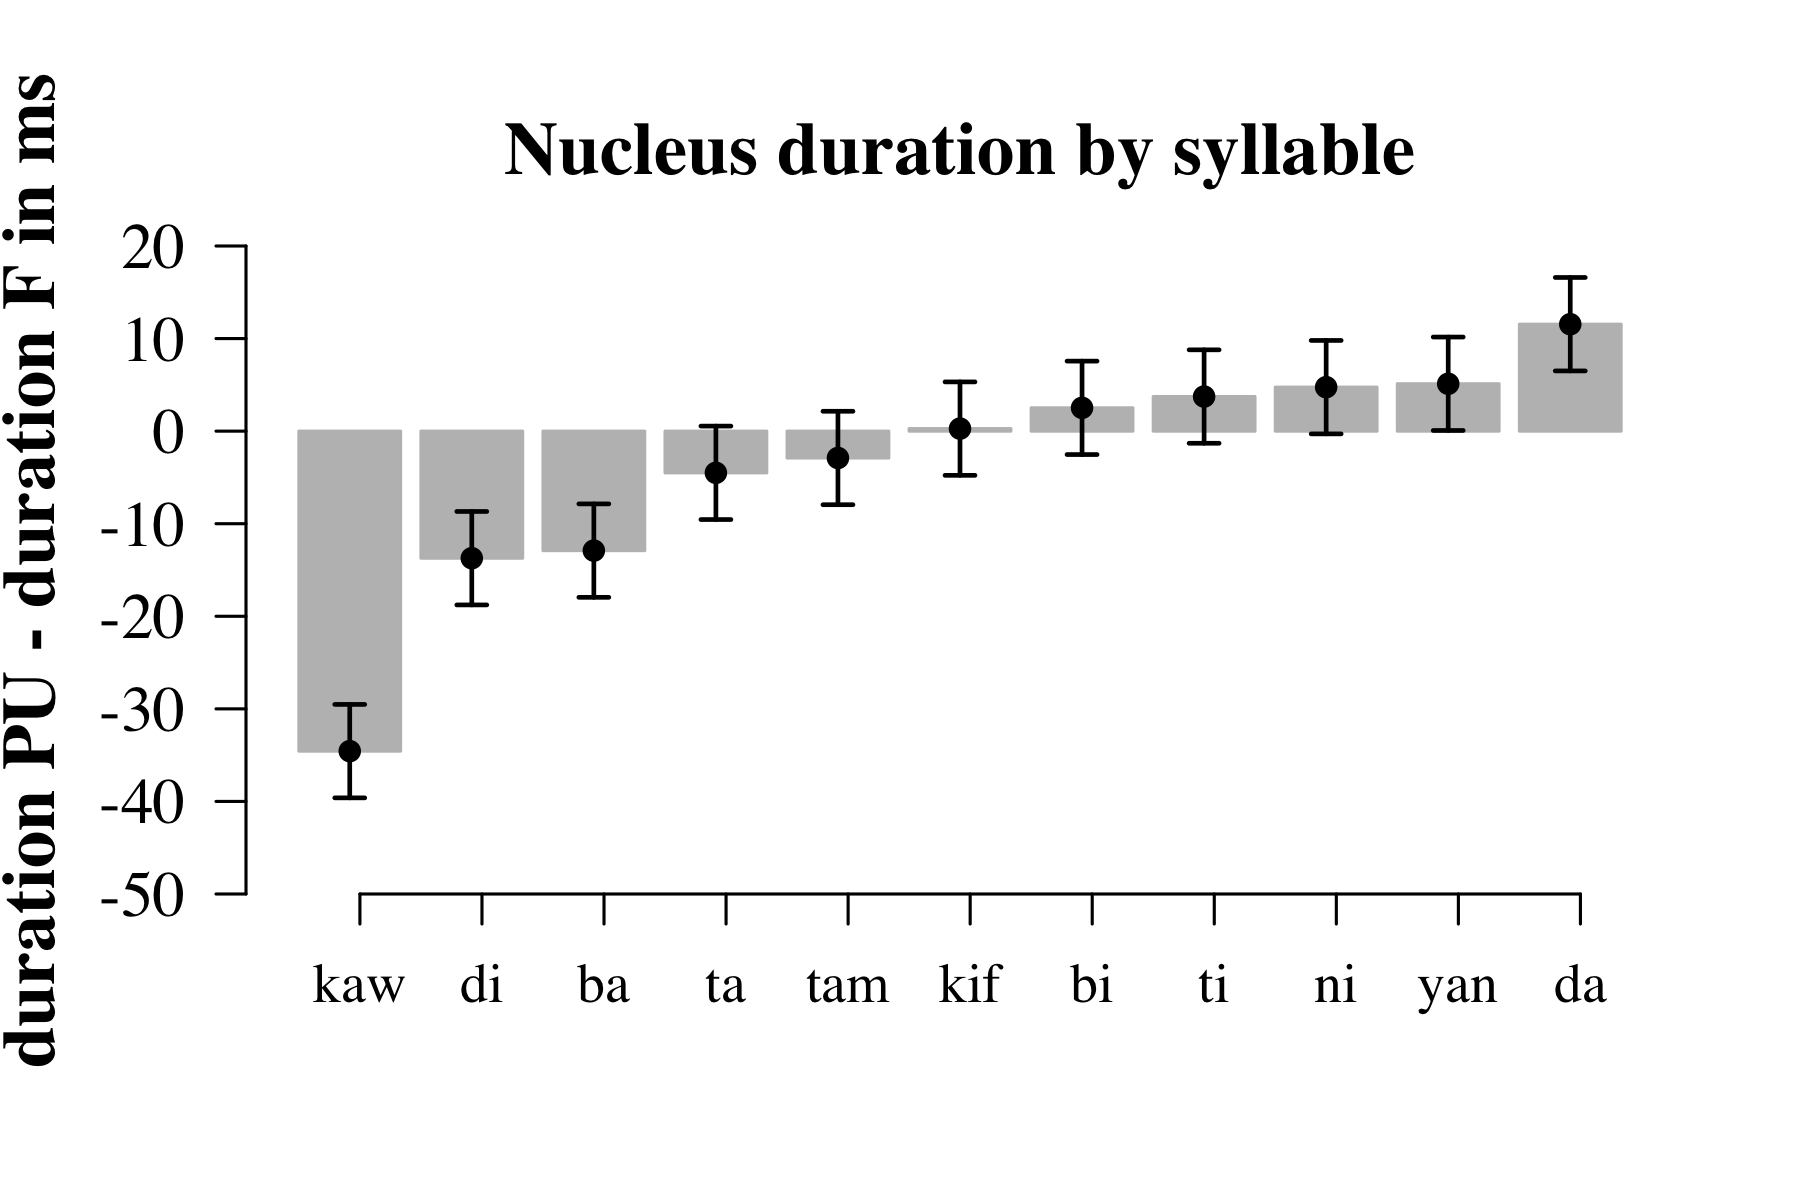
\includegraphics[trim={0 3cm 0 0}, clip, width=0.9\textwidth]{figures/Figure_4_2.png}
  \caption{Difference scores of vowel duration of penult (PU) minus final syllable (F). Means are arranged according to magnitude for all target syllables. Negative values indicate greater duration for the F; positive values indicate greater duration for the PU. Error bars indicate standard errors taken from the model described above.}
   \label{fig:4.2}
   \end{figure}

\begin{figure}
  \centering 
   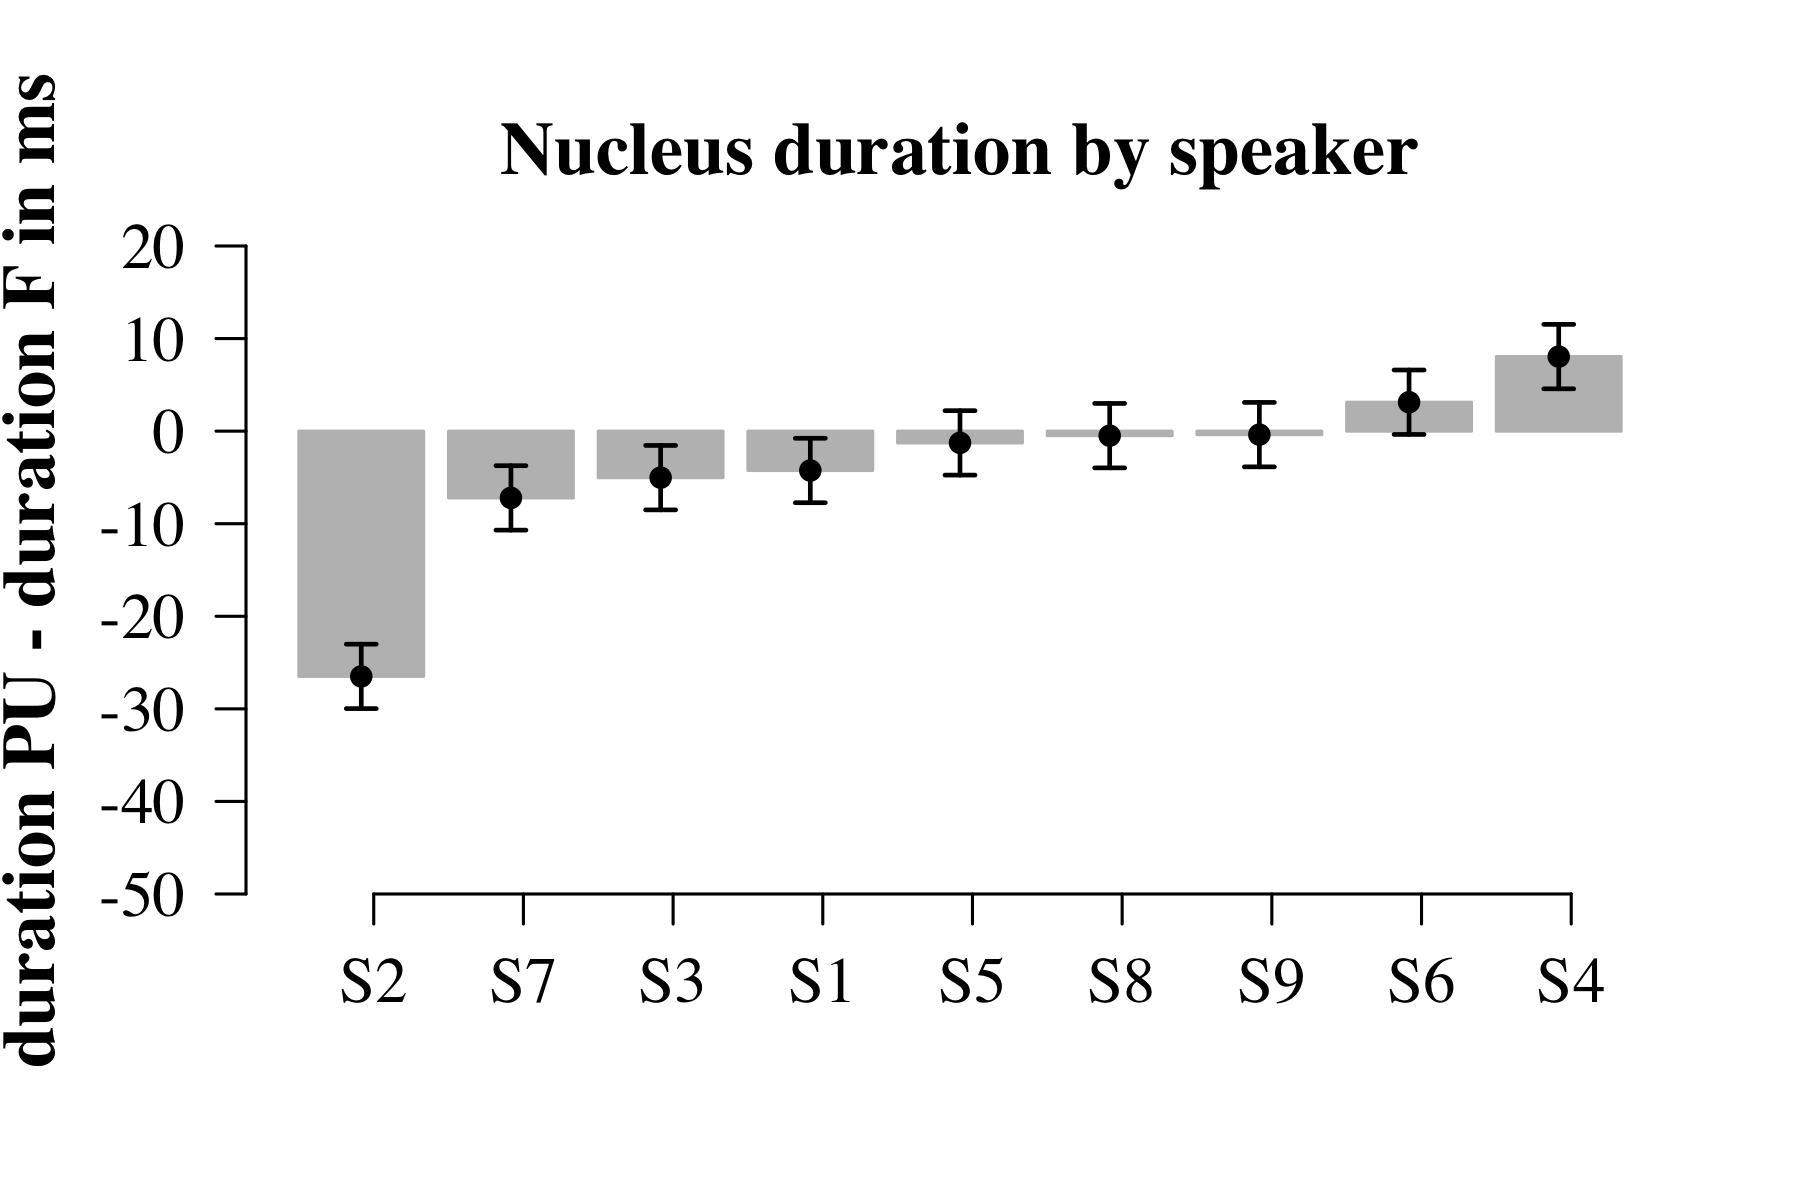
\includegraphics[trim={0 3cm 0 0},width=0.9\textwidth]{figures/Figure_4_3.png}
  \caption{Difference scores of vowel duration of penult (PU) minus final syllable (F). Means are arranged according to magnitude for all speakers. Negative values indicate greater duration for the F; positive values indicate greater duration for the PU. Error bars indicate standard errors taken from the model described above.}
   \label{fig:4.3}
   \end{figure}

\subsubsection{Intensity}
Looking at the intensity patterns displayed in Figures \ref{fig:4.4} and \ref{fig:4.5}, a slightly different picture emerges. Again, intensity is given as the difference between the mean intensity of the target syllable nucleus in penultimate position and final position. Eight of eleven target syllables and six of nine speakers have positive values indicating higher intensity in the penultimate vowel. This descriptive trend goes in the opposite direction of the trend that Gordon and Nafi reported in their study. While these trends do not hold for the subject-based model inferentially (β=0.36, SE=0.31, χ\textsuperscript{2}(1)=1.43, p=0.23), there is in fact a significant effect for the syllable-based analysis (β=0.5, SE=0.18, χ\textsuperscript{2}(1)=6.03, p=0.014). 

\begin{figure}
  \centering 
   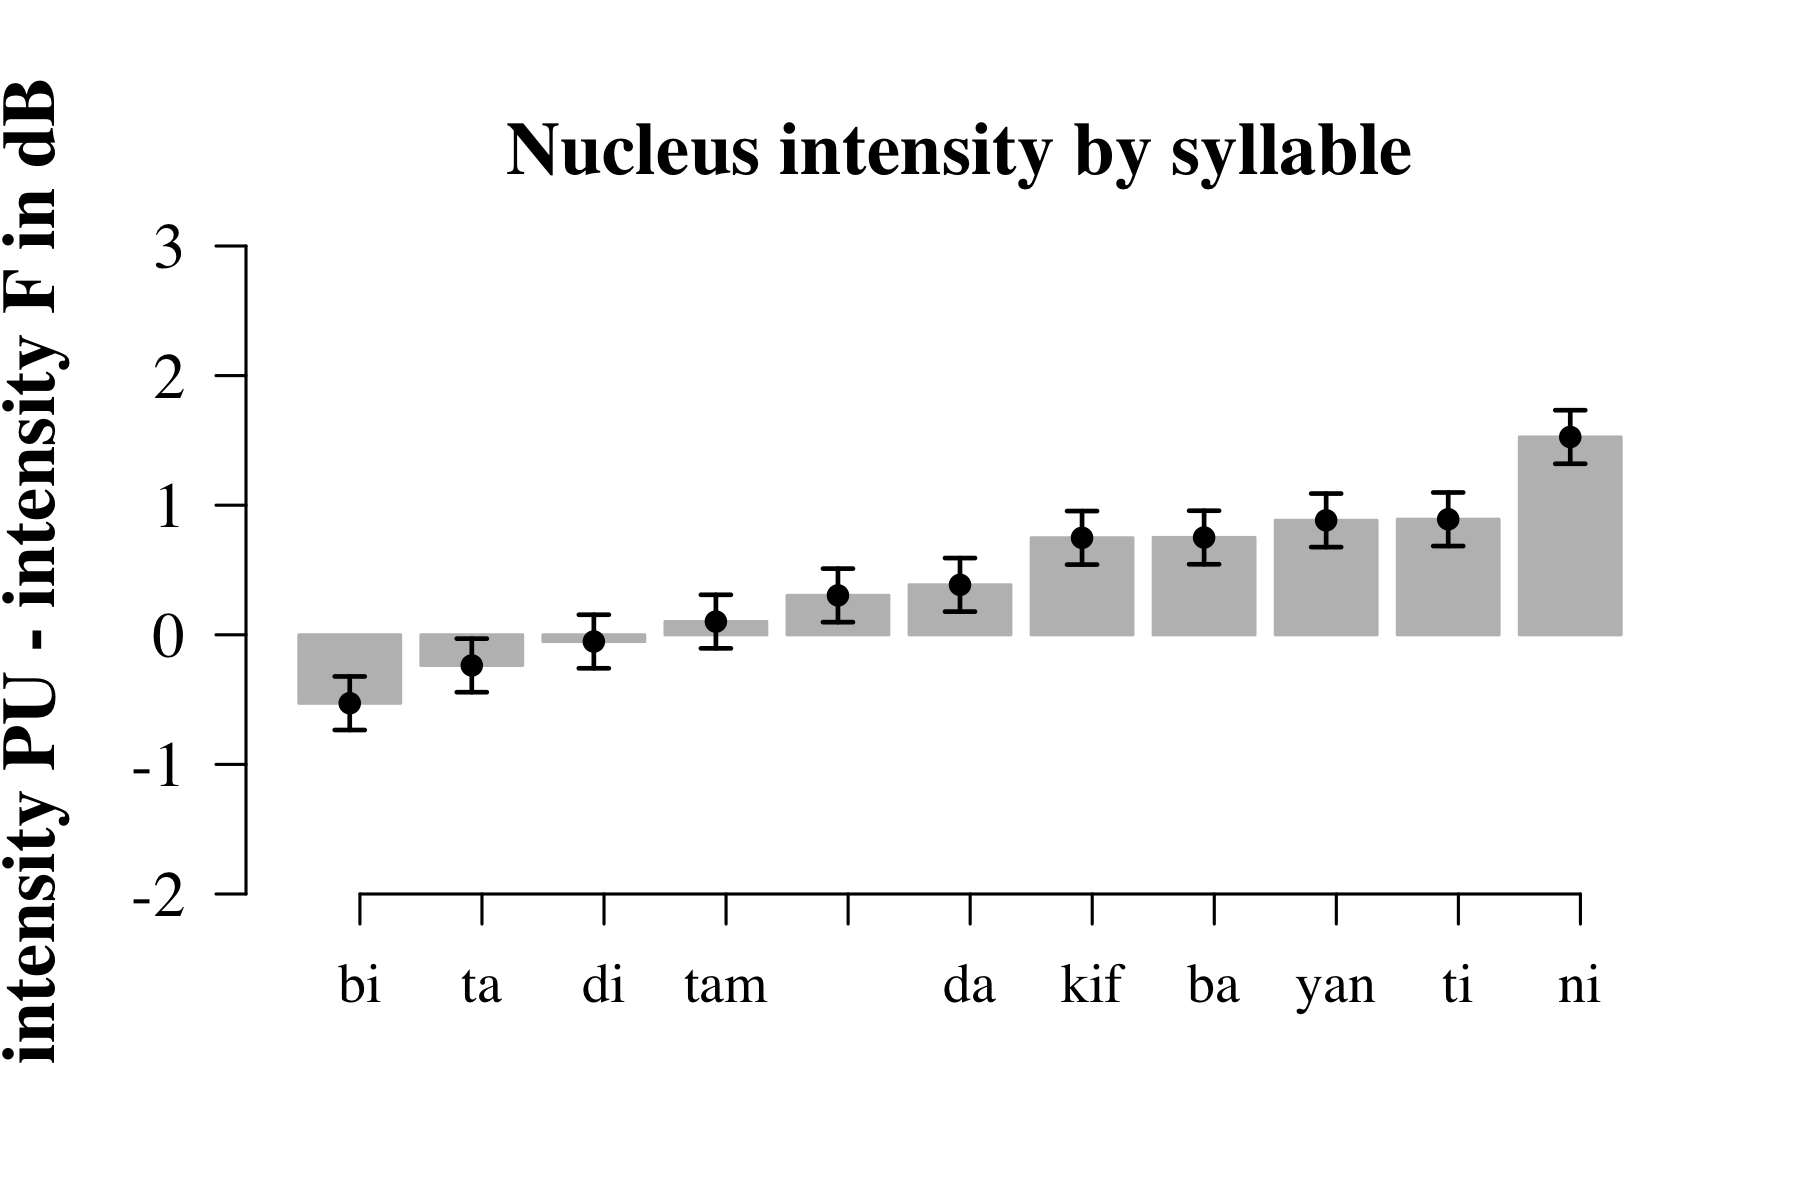
\includegraphics[trim={0 3cm 0 0},width=0.9\textwidth]{figures/Figure_4_4.png}
  \caption{Difference scores of vowel intensity of penult (PU) minus final syllable (F). Means are arranged according to magnitude for all target syllables. Negative values indicate greater intensity for the F; positive values indicate greater intensity for the PU. Error bars indicate standard errors taken from the model described above.}
   \label{fig:4.4}
   \end{figure}

\begin{figure}
  \centering 
   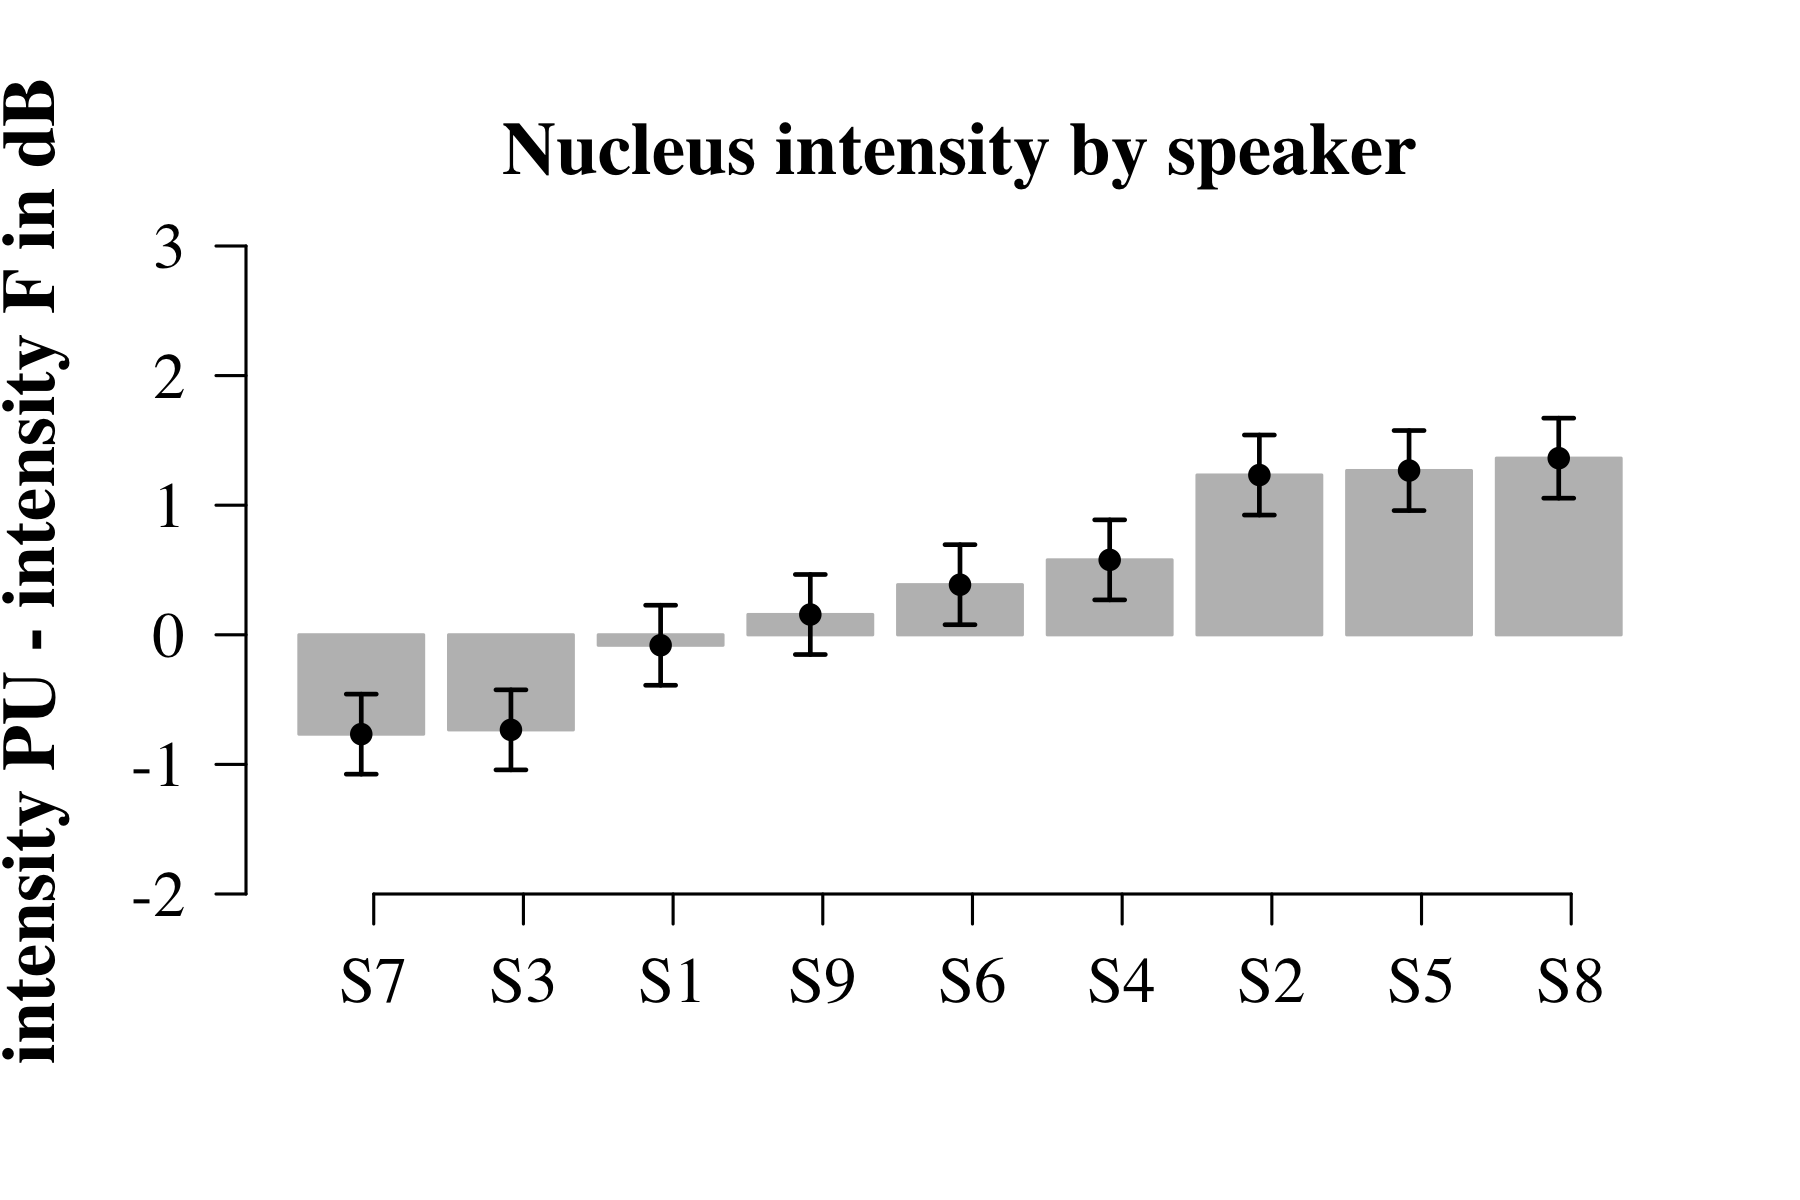
\includegraphics[trim={0 3cm 0 0},width=0.9\textwidth]{figures/Figure_4_5.png}
  \caption{Difference scores of vowel intensity of penult (PU) minus final syllable (F). Means are arranged according to magnitude for all speakers. Negative values indicate greater intensity for the F; positive values indicate greater intensity for the PU. Error bars indicate standard errors taken from the model described above.}
   \label{fig:4.5}
   \end{figure}

Despite exhibiting a statistically significant effect, there are three arguments against the assumption that these differences are linguistically relevant. First, the estimation of the effect size is 0.36 dB and 0.5 dB, for the subject-based and syllable-based models, respectively. These values clearly lie below the commonly assumed just noticeable difference\is{just noticeable difference} of 1 dB for intensity (cf. \citealt[119]{Lehiste1970}). This average difference, thus, is unlikely to be used by listeners as a perceptual cue to stress.

Second, the consistent trend for louder syllables in the penult may be an artefact of a general declination of intensity throughout the utterance. This general trend has been observed for other languages (\citealt{Ladefoged1972,LiebermanBlumstein1988,VayraFowler1992}) and is apparent in other data sets of Tashlhiyt (impressionistic observation by the author). This intensity declination, however, might not be as robust across the speaker population, explaining the lack of a significant effect in the subject-based analysis. \is{declination}

To explore whether the effect of intensity could be due to intensity declination, utterances were divided into ten equally long intervals. For each interval, the intensity mean was extracted. Intensity values were then submitted to statistical analysis. Intensity was modeled as a function of time steps (1-10). Both subject-based (averaging over target words) and item-based (averaging over subjects) analyses were performed. Both the subject-based (β=-0.68, SE=0.11, χ\textsuperscript{2}(1)=31.2, p<0.00001), and the item-based analysis (β=-0.68, SE=0.07, χ\textsuperscript{2}(1)=79.1, p<0.00001) showed a significant negative linear trend, i.e. intensity decreases throughout the utterance by an estimated 0.7 dB from one step (1/10 of the utterance) to the next.\is{declination}

\begin{figure}
  \centering 
   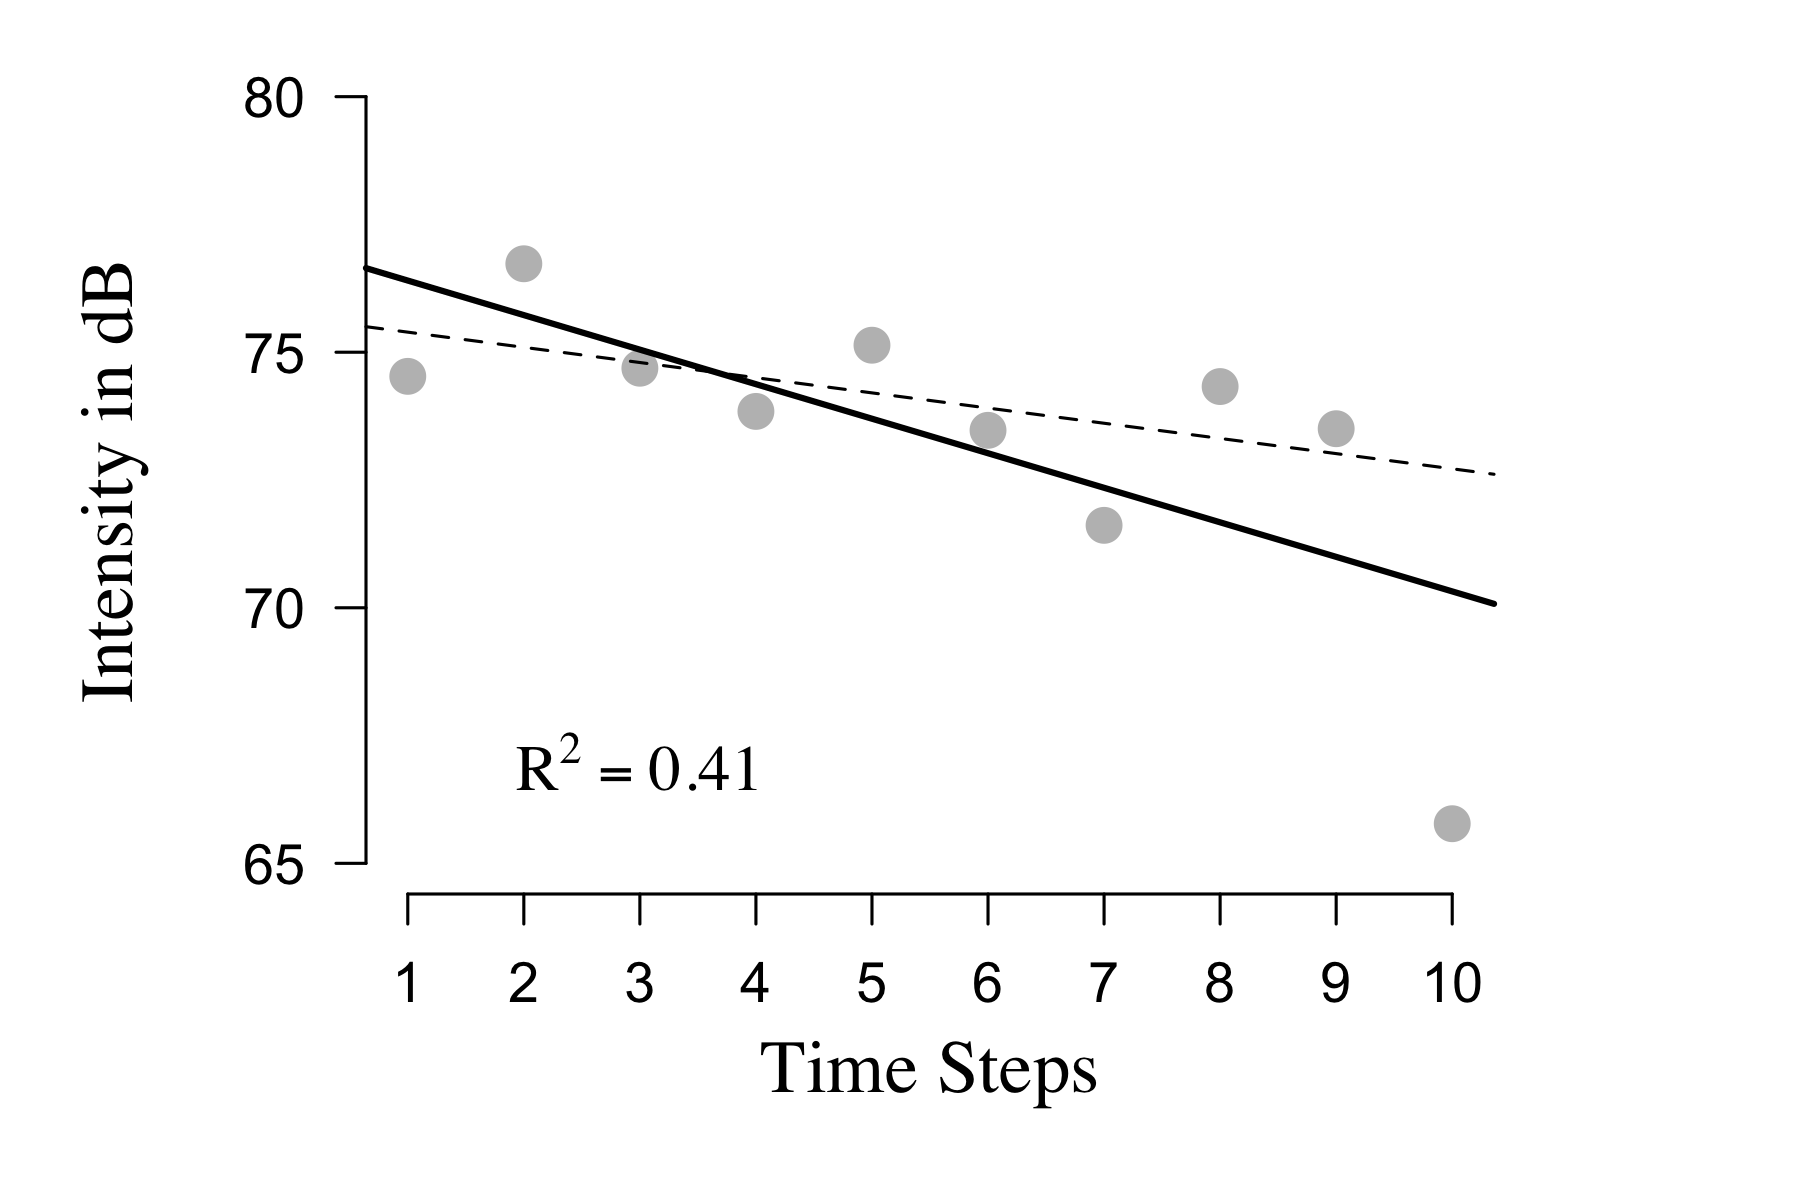
\includegraphics[trim={0 3cm 0 0},width=0.8\textwidth]{figures/Figure_4_6.png}
  \caption{Aggregated mean intensity values as a function of time and the corresponding regression line (solid line). The R\textsuperscript{2} value corresponds to the adjusted explained variance of the solid line. The dashed line indicates the negative trend excluding the final intensity value.}
   \label{fig:4.6}
   \end{figure}

\figref{fig:4.6} illustrates the negative linear trend throughout the utterance (averaging across both speakers and words). Note that this trend is not an artefact of a sudden drop in intensity at the end of the utterance (although it is certainly influenced by it). Even though the estimated negative trend is clearly smaller after excluding time step 10 (β=0.35, corresponding to the dashed line in \figref{fig:4.6}), it is still significantly negative indicating a decreasing trend in intensity. The effect size from one time step to the next (0.35 dB) numerically corresponds to the estimated difference between the penult and the final syllable in the analysis performed above (0.36 dB for subjects and 0.5 dB for syllables). Thus, this global downdrift likely accounts for the intensity asymmetries between penult and final syllables. We conclude that the asymmetry found above is unlikely to be the result of lexically specified prominence asymmetries. The effect size is too small to be considered a perceptually relevant cue and better corresponds to a global declination trend across the entire utterance.\is{declination}

Third, applying a more conservative statistical analysis to the intensity patterns across syllable positions including crossed by-subject and by-syllable random slopes, the significant effect vanishes. There remains no statistically generalisable effect of intensity predicted by syllable position (β=0.36, SE=0.27, χ\textsuperscript{2}(1)=1.9, p=0.17).

\subsubsection{Fundamental frequency (f0)}
Finally, we consider mean fundamental frequency of the vowels in the target syllable. In Figures \ref{fig:4.7} and \ref{fig:4.8}, fundamental frequency is given as the difference between the mean fundamental frequency of the target syllable nucleus in penultimate position and final position. The plot clearly indicates a consistent asymmetry across syllables and speakers. The penultimate syllable has on average 9 Hz higher mean f0 values than the final syllable. This asymmetry is significant for both the subject-based and syllable-based analyses (β≤9.55, SE≥1.97, χ\textsuperscript{2}(1)≤4.6, p≤0.03). Applying a more conservative statistical analysis including crossed by-subject and by-syllable random slopes, the significance of the effect remains robust (β=11.6, SE=3.9, χ\textsuperscript{2}(1)=6.8, p=0.009).

\begin{figure}
  \centering 
   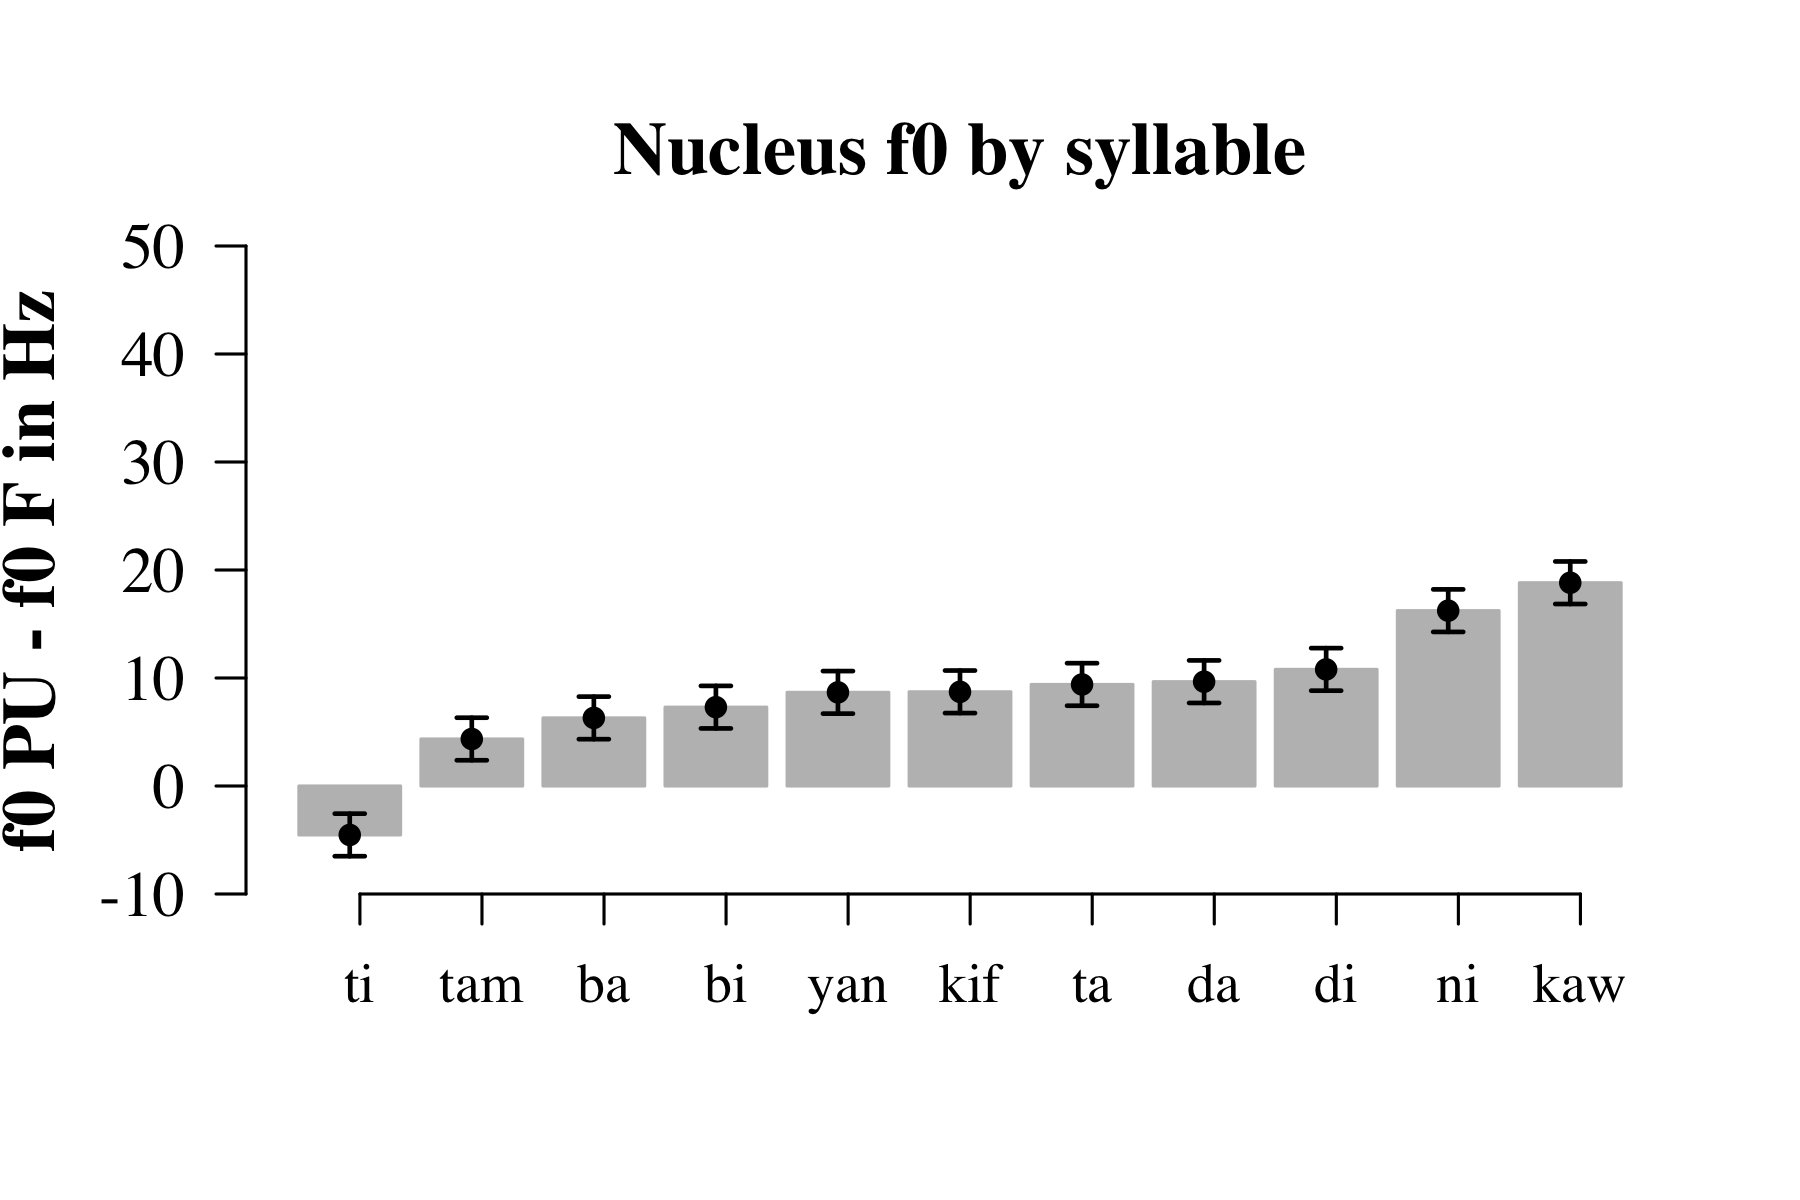
\includegraphics[trim={0 5cm 0 0},width=0.9\textwidth]{figures/Figure_4_7.png}
  \caption{Difference scores of fundamental frequency (f0) of penult (PU) minus final syllable (F). Means are arranged according to magnitude for all target syllables. Negative values indicate greater f0 for the F; positive values indicate greater f0 for the PU. Error bars indicate standard errors taken from the model described above.}
   \label{fig:4.7}
   \end{figure}

\begin{figure}
  \centering 
   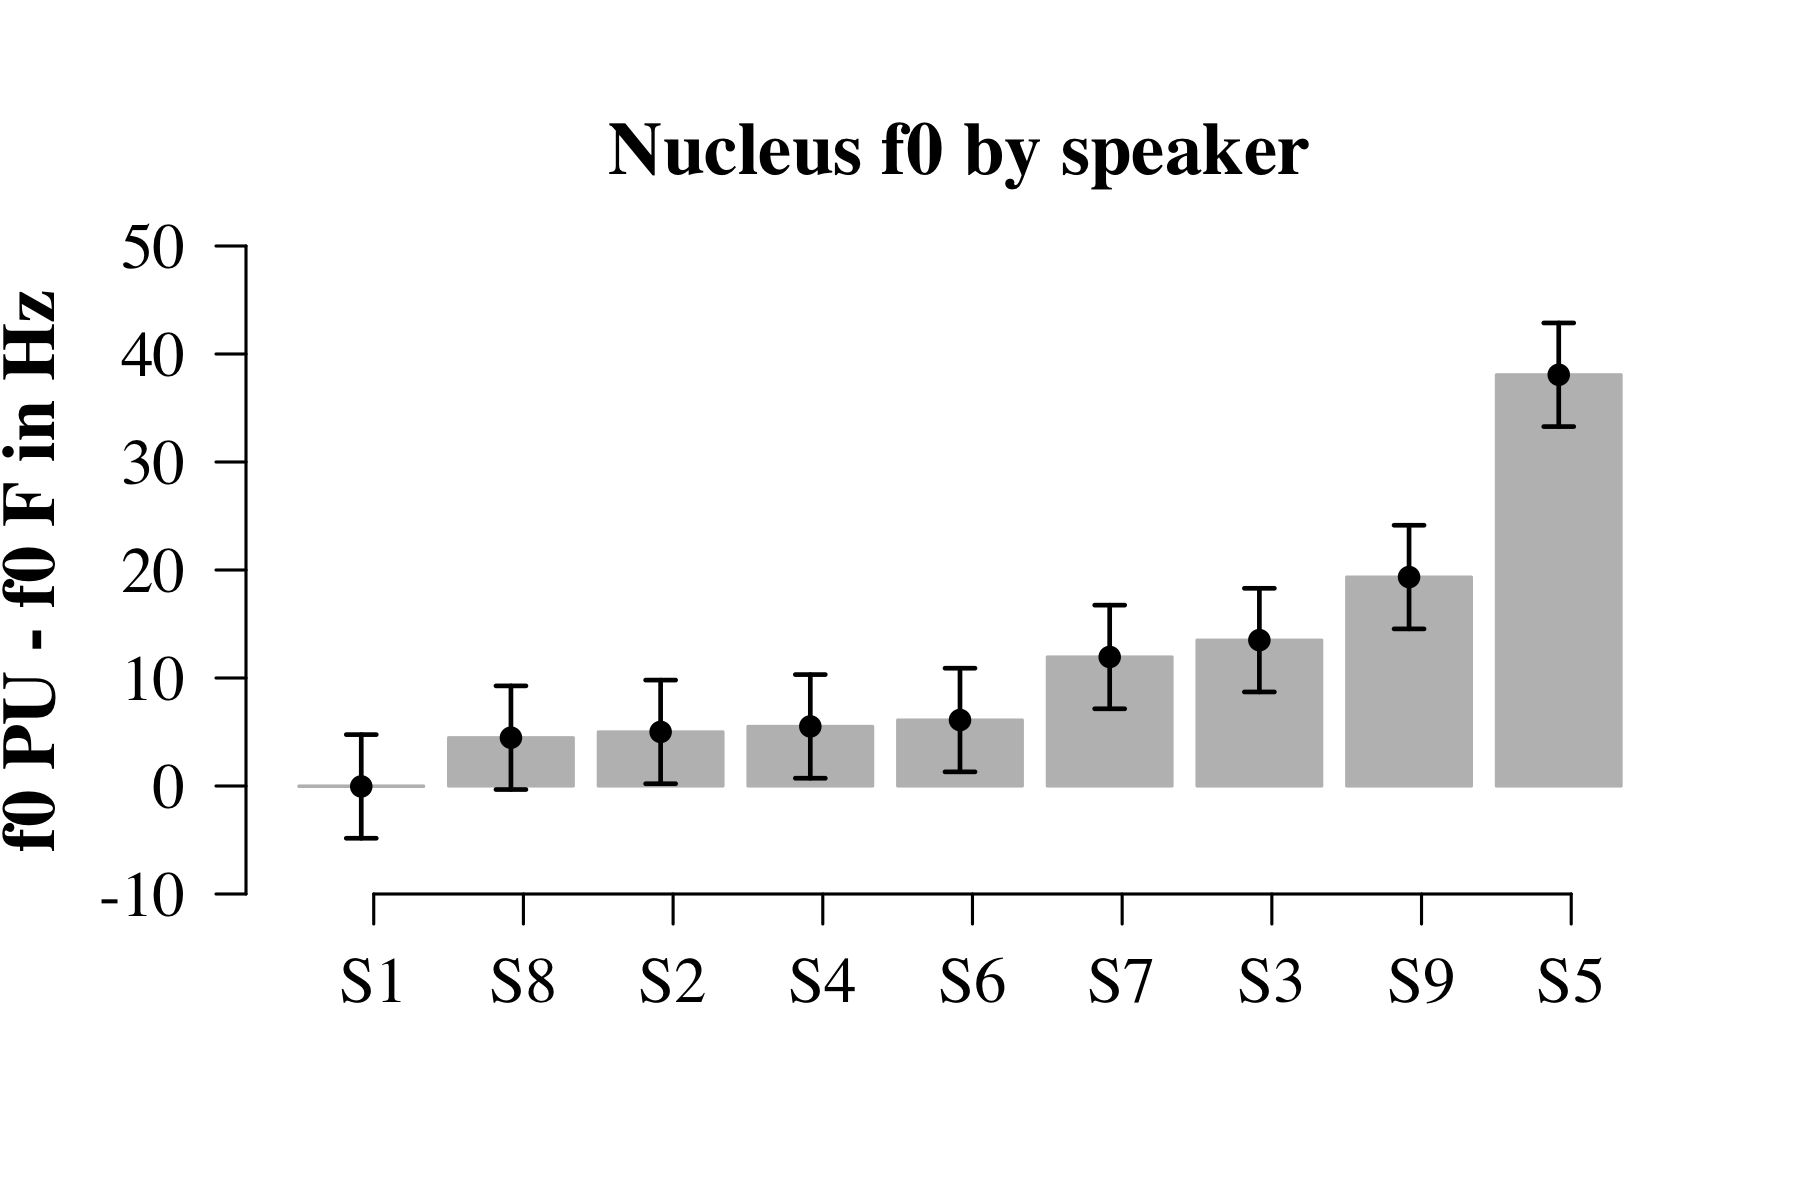
\includegraphics[trim={0 5cm 0 0},width=0.9\textwidth]{figures/Figure_4_8.png}
  \caption{Difference scores of fundamental frequency (f0) of penult (PU) minus final syllable (F). Means are arranged according to magnitude for all speakers. Negative values indicate greater f0 for the F; positive values indicate greater f0 for the PU. Error bars indicate standard errors taken from the model described above.}
   \label{fig:4.8}
   \end{figure}

This consistent but subtle f0 difference may be an artefact of two confounding factors. First, there were strong microprosodic influences of the voiced uvular fricative of /ʁakudan/ following the final target syllable. This leads to a drop in f0 as is illustrated in \figref{fig:4.1}. Second, there was a general declination trend of f0 from the beginning of the utterance towards the low pitch target preceding the sharp rise at the end of the phrase. Even though the stimuli were chosen so as not to exhibit phrasal effects, utterance-wide declination trends can be observed that result in consistent, but numerically subtle differences in f0.\is{microprosody}\is{declination}

\subsubsection{Discussion}
In sum, the null hypothesis for the assumption of fixed word stress cannot easily be rejected based on descriptive or inferential grounds. There are no acoustic prominence asymmetries between syllables of any given target word in a consistent manner across items or speakers. If anything, descriptive trends and a significant syllable-based analysis point to louder vowels in the penult (as opposed to louder vowels in the final syllable as found in \citealt{GordonNafi2012}). This intensity effect, however, is below the just noticeable difference threshold, the magnitude of the effect corresponds to a general declination of intensity throughout the utterance, and more conservative statistical analyses do not support the generalisability of this effect. Pitch shows a consistent effect of lower pitch values on the final syllable. This effect is of low magnitude and probably an artefact of independent segmental perturbations. Taken together, the evidence presented here casts reasonable doubt on the claim that Tashlhiyt exhibits word stress as reflected in prominence asymmetries.\is{microprosody}\is{declination}\is{just noticeable difference}

While Tashlhiyt often gives the impression that one syllable is more prominent than neighbouring syllables within the word, this impression quickly fades after hearing other instances of the same word produced by the same speaker. The observed patterns in Tashlhiyt resonate well with the following quote on the Salish language Nuxalk\il{Nuxalk}, often referred to as Bella Coola.

\begin{indentquote}{1.5em}
 [In Bella Coola there are] … no phonemically significant phenomena of stress or pitch associated with syllables or words… When two or more syllabics occur in a word or a sentence, one can clearly hear different degrees of articulatory force. But these relative stresses in a sequence of acoustic syllables do not remain constant in repetitions of the utterance (\citealt[132]{Newman1947}, cited after \citealt[57]{Hyman2014})
\end{indentquote}

Taken together, these findings lead to a rejection of the very specific claim that Tashlhiyt exhibits acoustic prominence asymmetries at the word level (\citealt{GordonNafi2012}). The assumption of word stress in Tashlhiyt was only based on Gordon and Nafi’s acoustic results. Given that this chapter showed that their results do not replicate and that there are no other phonological arguments for word stress, the general claim that Tashlhiyt exhibits word stress needs to be rejected until further evidence is found to the contrary.

\section{Summary}\label{sec:4.4}
Given the present findings, there is no evidence for prominence asymmetries in words containing vowels. Neither duration nor intensity differ across syllable positions. Pitch is generally slightly lower on the final syllable, but this has been argued to be due to microprosody and global declination. Placing these results in a wider context, a number of studies have argued against the presence of word stress in other languages. Three studies that are of particular interest are sketched here: \citet{MaskGussenhoven2016} argue that Ambonese Malay lacks word stress (see also \citealt{GoedemansZanten2007}, for evidence on Indonesian\il{Indonesian}). They looked at pitch peak alignment in phrase-final words and were unable to identify a stable landmark that serves as an anchor for the high tone. Moreover, they show that phonetic prominence asymmetries can be attributed to aspects of higher order prosodic organisation, i.e. durational asymmetries are attributed to domain-final lengthening. The latter finding emphasises the methodological relevance of disentangling postlexical aspects of speech from lexical ones (\citealt{Gordon2014,RoettgerGordon.underreview}). \is{word stress}\is{microprosody}\is{declination}\il{Malay (Ambonese)}

Another language reportedly lacking word stress is Tamil. Tamil has been described as having no distinctive word-level prominence, however, the literature anecdotally reports on the special status of the word-initial syllable. \citet{Keane2006} carried out an acoustic study to address this issue. Her data, based on five speakers, showed no consistent acoustic asymmetry across syllable positions, neither in duration nor in intensity. Interestingly, Keane presents the results for different words descriptively, and, similar to Tashlhiyt, there are large differences across different syllables with some syllables being longer in word-initial position and others being longer in word-medial position. However, initial syllables are consistently produced with a rising tone, which may be interpreted as evidence for fixed word stress. However, as Keane rightly acknowledges, this rising tone may instead be a postlexical tone that is aligned to the left edge of a prosodic constituent smaller than the intonation phrase.\il{Tamil}

Finally, \citet{brunelle2017} discusses word stress in Southern Vietnamese. The literature has made contradicting claims about whether Vietnamese can be described as having word stress or not and if so where in the word it is. Brunelle provides acoustic evidence suggesting that there is little evidence for word stress in Southern Vietnamese and that earlier reports of final stress are best interpreted as an artefact of higher prosodic structure, i.e. phrase-final lengthening.\il{Vietnamese}

These three case studies highlight the potential confounding of word stress and postlexical structure. As discussed at the beginning of this chapter, many studies reporting on word prosodic systems have used a methodology that did not allow for the disentangling of word-level and phrase-level phenomena. \citet{RoettgerGordon.underreview} confirm this impressionistic observation based on a corpus of more than 100 studies investigating over 70 languages. \citet{Gordon2014} points to this threat in prosodic research: 

\begin{quote}
 […] a large portion, if not the majority, of the prosodic typology that is currently understood to refer to stress may actually reflect phrasal prominence associated with tonal events occurring at or near phrasal edges. (\citealt[111]{Gordon2014})
\end{quote}

The present chapter argued for the absence of acoustic reflexes of phonological word stress in Tashlhiyt by carefully controlling for such confounds. At present, there is no convincing phonetic or phonological evidence for the presence of word stress in Tashlhiyt.

In the following chapters, higher prosodic aspects of the language will be investigated. Findings will show that the placement of intonational events flagging questions and marking contrastive constituents are prone to a vast amount of variation, lending additional support to the conclusion that there is no word stress in Tashlhiyt. 

